\documentclass[%
  aip,
  amsmath,amssymb,
  reprint,
  showkeys,
  % linenumbers, % Temporarily disabled in the reading version.
]{revtex4-1}

% --------------------------
% Core REVTeX/AIP packages
% --------------------------
\usepackage{graphicx} % Include figure files
\usepackage{dcolumn}  % Align table columns on decimal point
\usepackage{bm}       % bold math

% --------------------------
% Encoding / fonts
% --------------------------
\usepackage[utf8]{inputenc}
\usepackage[T1]{fontenc}

% Times 系列字体：二选一。
\usepackage{mathptmx}
% \usepackage{times} % 

% --------------------------
% Math / symbols (REVTeX 已通过 class 选项加载 amsmath, amssymb，这里不再重复加载)
% --------------------------
\usepackage{amsfonts}
\usepackage{mathrsfs}

% --------------------------
% Tables
% --------------------------
\usepackage{booktabs}
\usepackage{makecell}
\usepackage{siunitx}

% --------------------------
% Utilities
% --------------------------
\usepackage{etoolbox}
\usepackage{soul}
\usepackage{wrapfig}
\usepackage{xcolor}
\usepackage{float}
\usepackage{algorithm}
\usepackage{algorithmic}
\usepackage[hidelinks]{hyperref}
% Keep lineno loaded so auxiliary files from numbered drafts remain readable.
% Loading the package does not activate line numbering.
\usepackage{lineno}
\AtBeginDocument{\nolinenumbers}
% Frontiers in Physics uses numbered citations in square brackets.
\AtBeginDocument{\setcitestyle{numbers,square,comma}}
% Do not stretch paragraph and equation spacing to align column bottoms.
\raggedbottom


%% Apr 2021: AIP requests that the corresponding
%% email to be moved after the affiliations
\makeatletter
\def\@email#1#2{%
 \endgroup
 \patchcmd{\titleblock@produce}
  {\frontmatter@RRAPformat}
  {\frontmatter@RRAPformat{\produce@RRAP{*#1\href{mailto:#2}{#2}}}\frontmatter@RRAPformat}
  {}{}
}%

\makeatletter
\def\switch@array{}
\makeatother

\begin{document}



\title[]{Environment-dependent peer pressure with reinforcement learning promotes cooperation in spatial public goods games}
% Force line breaks with \\




\author{Author name}
% \date{\today}% It is always \today,

\begin{abstract}
Cooperation evolution in social dilemmas has been widely studied, with social influence mechanisms providing important explanations for the emergence and maintenance of cooperation. Among these mechanisms, peer pressure shapes individual behaviors. However, the interaction between peer pressure and individual learning under different local behavioral environments remains to be clarified. To address this, we propose an environment-dependent peer pressure mechanism combined with an environment-aware reinforcement learning framework in a spatial public goods game. Our results show that the effect of peer pressure on cooperation evolution depends on its intensity, the synergy factor, and the environmental threshold. Under representative conditions, moderate pressure promotes cooperation, whereas excessive pressure disrupts cooperative dynamics and eventually leads to the collapse of cooperation. Moreover, incorporating both individual behavior and group environment into the learning state supports higher cooperation than either simplified state representation under the examined conditions. This study highlights the importance of adaptive social feedback and learning processes in understanding cooperation evolution in complex systems.
\end{abstract}

\keywords{evolution of cooperation; spatial public goods game; peer pressure; reinforcement learning; environmental feedback; state representation}



\maketitle

\noindent{\small Main-text word count: approximately 3252; Figures: 6; Tables: 0.}\par

\section{\label{sec:level1}INTRODUCTION}

Cooperation is a fundamental phenomenon widely observed in biological and social systems~\cite{rand2013human,axelrod1981evolution}, ranging from microbial communities to human societies. 
However, cooperation remains a challenging phenomenon from the perspective of Darwinian natural selection, because cooperative behaviors require individuals to bear additional costs while the resulting collective benefits may also be exploited by others~\cite{sigmund2010calculus}. 
Understanding how cooperation can emerge and persist despite the potential advantages of selfish behaviors has therefore become a central topic in social science~\cite{pennisi2005did}.

Evolutionary game theory provides a framework for investigating the mechanisms underlying cooperation~\cite{smith1973logic,taylor1978evolutionary}. 
Among various theoretical models, the public goods game has been widely used to characterize social dilemmas in which individuals must decide whether to contribute to collective benefits~\cite{hauert2006evolutionary,kurokawa2009emergence,szolnoki2016competition}. 
In particular, spatial public goods games incorporate population structure and local interactions into evolutionary models, allowing researchers to investigate how spatial organization and neighborhood interactions influence cooperative dynamics~\cite{quan2018continuous,yang2018benefits,szolnoki2009impact,perc2013evolutionary}. 
Previous studies have shown that spatial structure and various social mechanisms can affect the evolution of cooperation~\cite{nowak1992evolutionary,ohtsuki2006simple,perc2010coevolutionary,perc2017statistical,nowak2006evolutionary}. 
However, cooperation remains vulnerable to exploitation by non-cooperative behaviors~\cite{olson1971logic}, motivating extensive investigations into mechanisms that can stabilize cooperation, including punishment~\cite{fehr2002altruistic,chen2014probabilistic,xie2024regulation,szolnoki2017antisocial,zhao2024emergence}, reward~\cite{david2009positive,wang2023synergistic}, reputation~\cite{milinski2002helps,santos2018social,ren2024interaction}, and environmental feedback~\cite{weitz2016oscillating,tilman2020evolutionary,wang2020eco}.

Peer pressure is an important social mechanism that can influence cooperative behaviors because individuals adjust their actions according to prevailing social norms~\cite{yang2015peer,deng2018peer}. 
Individuals who violate local behavioral expectations may experience disapproval, exclusion, or other forms of social pressure, leading them to adjust their behaviors toward prevailing patterns~\cite{asch1952social}. 
Previous studies have examined how peer pressure influences cooperation under different interaction and feedback mechanisms~\cite{hu2021peer,gao2023impact,ma2025evolution,xu2026synergistic}. 
In reality, the same behavior may receive different social feedback under different local conditions~\cite{zhu2024synergy,hu2025dynamic}. 
For example, in environmental conservation, individuals who refuse to participate in recycling or energy-saving activities may face social disapproval when such behaviors have become established local norms. 
Conversely, when environmentally responsible behaviors are not yet widely accepted, individuals who actively practice conservation may receive limited social support because their actions deviate from prevailing behaviors~\cite{cialdini1990focus}. 
Therefore, peer pressure should not be considered as a uniform social force, but rather as an environment-dependent feedback mechanism whose effects depend on local behavioral conditions.

This perspective motivates us to investigate how environment-dependent peer pressure regulates the evolution of cooperation. 
Answering this question requires not only understanding how social pressure is generated, but also considering how individuals perceive and respond to changing environmental conditions. 
Evolutionary game models describe strategy updating through payoff comparison or imitation~\cite{szabo2007evolutionary,traulsen2010human}. 
However, real decision-making processes are adaptive, with individuals acquiring information from their surroundings, evaluating the consequences of previous actions, and adjusting their future behaviors based on accumulated experiences~\cite{young2009learning}. 
Reinforcement learning provides a natural framework for describing such adaptive processes, where individuals learn appropriate behaviors through continuous interactions with their environments~\cite{mckee2023scaffolding,shi2024model,zheng2024evolution,koster2025deep,wang2025spatial,mintz2025evolutionary,lee2025granular,li2025cooperation,xie2026reinforcement,zheng2026brief}. 
By updating behavioral preferences according to received rewards, individuals can gradually adapt their strategies to changing conditions and establish feedback between behaviors and environmental states~\cite{shen2024adaptive,lv2025reinforcement,li2025environmental}.

In this work, we develop an environment-dependent peer pressure mechanism combined with reinforcement learning in a spatial public goods game. 
The proposed framework allows us to examine how social feedback changes under different environmental conditions. 
By integrating spatial interactions, environment-dependent social feedback, and individual learning, we investigate how social feedback and learning processes jointly shape the evolution of cooperation. 
Our results demonstrate that environment-dependent peer pressure can generate diverse evolutionary outcomes under different social conditions. 




\section{MODEL}\label{sec2}
\subsection{Spatial public goods game}

We consider a spatial public goods game on a square lattice with periodic boundary conditions. 
The population consists of $L \times L$ individuals, with each individual occupying a single lattice site. Each interaction group consists of a focal individual and its four nearest neighbors. 
Following the von Neumann neighborhood structure, each individual belongs to five overlapping groups, including the group centered on itself and the groups centered on its four neighboring individuals.

Each individual adopts one of two strategies, $\mathrm{C}$ and $\mathrm{D}$, where $\mathrm{C}$ denotes cooperation and $\mathrm{D}$ denotes defection. Thus, the strategy set is defined as $A=\{\mathrm{C},\mathrm{D}\}$.

In each public goods interaction, cooperators contribute a fixed cost $c=1$, whereas defectors contribute nothing. 
The total contribution from cooperators is multiplied by the synergy factor $r$ and equally distributed among all group members.

Therefore, the basic payoff obtained by individual $i$ in a group interaction is given by $\pi_i=\frac{rn_\mathrm{C}}{g}-c_i$, where $n_\mathrm{C}$ represents the number of cooperators in the group, $g=5$ is the group size, and $c_i=1$ if individual $i$ adopts cooperation and $c_i=0$ otherwise.


\subsection{Environment-dependent peer pressure mechanism}

We assume that peer pressure depends on the local environmental state of each interaction group. Specifically, the environmental state is determined separately for each group interaction according to the environmental threshold $T$. When the number of cooperators in the group satisfies $n_\mathrm{C}\geq T$, the interaction group is considered to be in a cooperative environment; otherwise, it is considered to be in a defective environment.

The environmental state determines which behavior is subjected to peer pressure. In a cooperative environment, defectors receive pressure from cooperators in the interaction group. In a defective environment, cooperators receive pressure from defectors in the group.

For individual $i$, the effective reward in a group interaction is defined as
\begin{equation}
R_i=\pi_i+P_i,
\label{eq:effective}
\end{equation}
where $\pi_i$ denotes the payoff obtained from the public goods game and $P_i$ represents the peer pressure term. The peer pressure term is defined as

\begin{equation}
P_i=
\begin{cases}
-\beta n_\mathrm{C}, & a_i=\mathrm{D},\ n_\mathrm{C}\geq T,\\
-\beta n_\mathrm{D}, & a_i=\mathrm{C},\ n_\mathrm{C}<T,\\
0, & \text{otherwise},
\end{cases}
\label{eq:pressure}
\end{equation}

where $n_\mathrm{D}=g-n_\mathrm{C}$ denotes the number of defectors in the interaction group, and $\beta$ represents the intensity of peer pressure. Here, $a_i$ denotes the action implemented by individual $i$ in the current interaction.

Through this formulation, peer pressure becomes an environment-dependent social influence mechanism whose effect depends on the prevailing behavioral environment. 
This allows us to investigate how individuals adapt their strategies as local group environments change and how environment-dependent social feedback influences the evolution of cooperation.


\subsection{Environment-aware reinforcement learning}

To describe how individuals adapt their behaviors under changing social environments, we introduce a Q-learning framework into the spatial public goods game.

Previous studies have used an individual's previous strategy to define its state~\cite{wang2022levy,fan2022incorporating,du2026shaping}. 
However, incorporating environmental information into the state representation allows individuals to distinguish group environments during learning~\cite{li2025environmental}. 
In our model, individual rewards depend on both their strategies and the surrounding social environment. 
Therefore, the state space is defined by the individual's current strategy and the environmental condition of the interaction group.

Combining these two components gives four states,
$s_1=(\mathrm{C},\mathrm{G})$,
$s_2=(\mathrm{C},\mathrm{B})$,
$s_3=(\mathrm{D},\mathrm{G})$,
and
$s_4=(\mathrm{D},\mathrm{B})$,
where $\mathrm{G}$ and $\mathrm{B}$ denote cooperative and defective environments, respectively.

For each individual, the Q-table records the expected discounted cumulative reward of each state-action pair and has the form

\begin{equation}
Q_i=
\begin{bmatrix}
Q_i(s_1,\mathrm{C})&Q_i(s_1,\mathrm{D})\\
Q_i(s_2,\mathrm{C})&Q_i(s_2,\mathrm{D})\\
Q_i(s_3,\mathrm{C})&Q_i(s_3,\mathrm{D})\\
Q_i(s_4,\mathrm{C})&Q_i(s_4,\mathrm{D})
\end{bmatrix},
\end{equation}

where the two columns correspond to the two possible actions, cooperation and defection.

\begin{figure}[htbp]
\centering
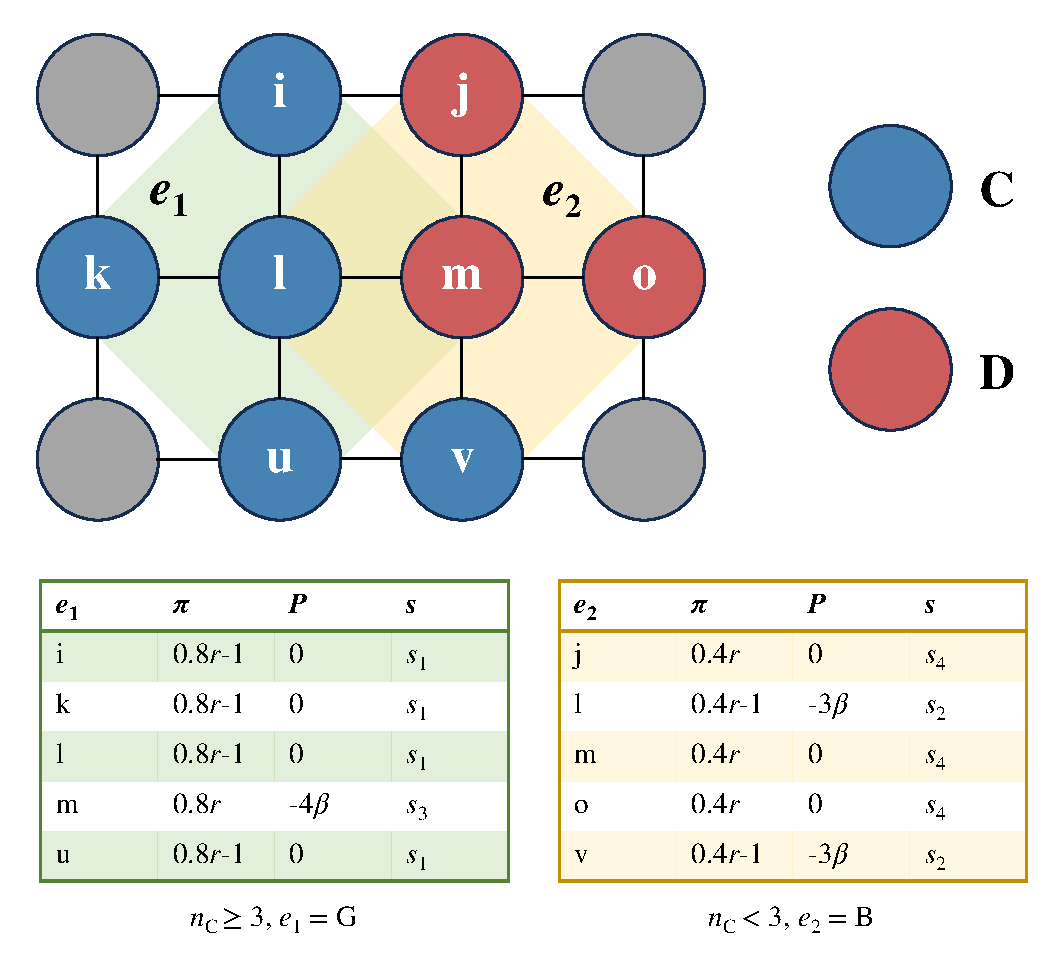
\includegraphics[width=\linewidth]{Fig_1.pdf}
\caption{
Illustration of payoff, peer pressure, and state assignment in two overlapping interaction groups under $T=3$. 
The left group $e_1$ is in the cooperative environment ($n_{\mathrm{C}}\geq T$), whereas the right group $e_2$ is in the defective environment ($n_{\mathrm{C}}<T$). 
The corresponding payoff $\pi$, peer pressure $P$, and state $s$ of each group member are shown in the tables.
}
\label{fig:Fig1}
\end{figure}

Figure~\ref{fig:Fig1} illustrates how the local environment determines the payoff, peer pressure, and state of each individual. 
For $T=3$, $e_1$ is classified as a cooperative environment ($\mathrm{G}$), whereas $e_2$ is a defective environment ($\mathrm{B}$). 
Because environmental states are determined separately for each interaction group, the same individual can have different states when participating in different overlapping groups.

At each decision-making step, individuals select their actions according to the $\epsilon$-greedy strategy. Specifically, they choose the action with the highest Q-value in the current state with probability $1-\epsilon$, while randomly selecting an action with probability $\epsilon$. When multiple actions have identical maximum Q-values, one action is randomly selected among them.

After interacting with neighbors, individuals receive the effective reward $R_i$, which incorporates both the material payoff from the public goods game and the social feedback generated by peer pressure. The Q-value is then updated according to the Q-learning rule

\begin{equation}
\begin{aligned}
Q_i(s_t,a_t)\leftarrow{}&Q_i(s_t,a_t)\\
&+\alpha\bigl[R_i(t)+\gamma\max_{a'}Q_i(s_{t+1},a')\\
&\hspace{2.7em}-Q_i(s_t,a_t)\bigr],
\end{aligned}
\label{eq:q-learning}
\end{equation}

where $\alpha$ denotes the learning rate and $\gamma$ represents the discount factor. 

Through this learning process, individuals continuously update their strategy preferences based on received rewards and perceived environmental conditions, allowing them to adapt their strategies under different social conditions.


\begin{algorithm}[H]
\caption{Pseudocode of spatial public goods game with environment-dependent peer pressure and Q-learning}
\label{alg:PGG_Qlearning}

\begin{algorithmic}[1]

\STATE \textbf{Input:} $L$, $r$, $T$, $\beta$, $\alpha$, $\gamma$, $\epsilon$

\STATE // Initialization

\STATE Initialize Monte Carlo simulation step $n$;

\FOR{each individual $i\in L\times L$}

    \STATE Initialize individual $i$'s strategy $\mathrm{C}$ or $\mathrm{D}$ randomly;

    \STATE Initialize Q-table elements to 0;

\ENDFOR

\STATE // Strategy interaction and learning

\FOR{each time step $t\in[1,n]$}

    \FOR{$L \times L$ interactions}

        \STATE Randomly select a focal individual $i$;

        \STATE Construct the interaction group consisting of $i$ and its four neighbors;

        \STATE Determine the current environmental state of the group;

        \FOR{each individual $j$ in the group}

            \STATE Get individual $j$'s current state $s_j$ based on strategy and environment;

            \IF{$prob < \epsilon$}

                \STATE Select an action randomly from $A=\{\mathrm{C},\mathrm{D}\}$;

            \ELSE

                \STATE Select the action with the highest Q-value in the current state;

            \ENDIF

        \ENDFOR

        \STATE Simultaneously implement the selected actions of all group members;

        \FOR{each individual $j$ in the group}

            \STATE Calculate individual $j$'s payoff $\pi_j$;
    
            \STATE Calculate peer pressure effect $P_j$ according to Eq.~(\ref{eq:pressure});
    
            \STATE Get effective reward $R_j$ according to Eq.~(\ref{eq:effective});
    
            \STATE Update individual $j$'s Q-table according to Eq.~(\ref{eq:q-learning});

        \ENDFOR

    \ENDFOR

\ENDFOR

\end{algorithmic}
\end{algorithm}


\subsection{Evolutionary process and simulation procedure}

We use a single group interaction as the elementary learning unit, rather than accumulating payoffs across overlapping groups~\cite{zhu2024synergy}. An individual can therefore update its action and Q-values multiple times within one Monte Carlo step (MCS) as it participates in different groups. Each update is conditioned on the environment of the corresponding interaction group~\cite{li2025environmental}.

Initially, each individual is randomly assigned a strategy of cooperation or defection, and all Q-values are initialized to zero. During each elementary interaction, a focal individual is randomly selected and forms an interaction group with its nearest neighbors through the public goods game. The environmental state of the interaction group is determined according to its cooperation level. Each group member then selects an action through the $\epsilon$-greedy strategy. All selected actions are implemented simultaneously, after which the group environment is reassessed. Each individual's next state is determined by its implemented action and the updated environment of the same interaction group. Each group member receives an effective reward that combines the public goods payoff and peer pressure effect, and updates its Q-table according to the Q-learning rule.

The above process is repeated until the system reaches a stationary state. The final cooperation level is calculated by averaging over the last $10^5$ MCS of a simulation lasting $10^6$ MCS. For parameter sets that do not reach a stationary state within $10^6$ MCS, the simulation is extended to $10^8$ MCS, and the average is taken over the last $10^7$ MCS. One MCS consists of $L^2$ elementary interactions, during which each individual is selected as the focal individual once on average. The detailed evolutionary process is summarized in Algorithm~\ref{alg:PGG_Qlearning}. Unless otherwise specified, the simulations are performed on a $100\times100$ lattice with learning parameters $\alpha=0.1$, $\gamma=0.9$, and $\epsilon=0.01$~\cite{zhao2024emergence,zheng2024evolution,li2025environmental}.




\section{Analysis of Results}\label{sec3}


\begin{figure*}[htbp]
\centering
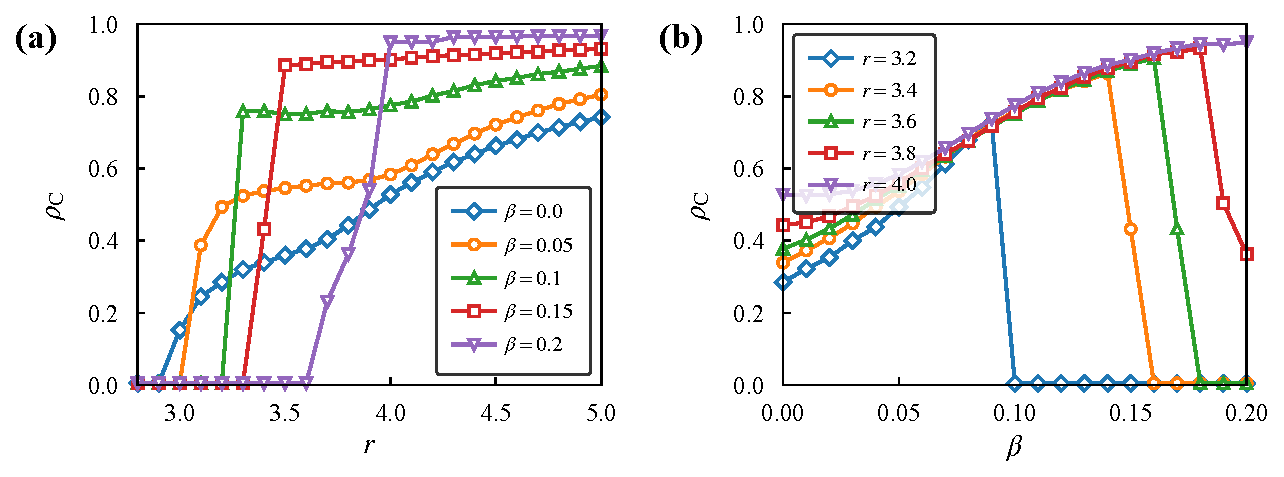
\includegraphics[width=\linewidth]{Fig_2.pdf}
\caption{
Effects of environment-dependent peer pressure on cooperation evolution.
(a) Final cooperation level $\rho_{\mathrm{C}}$ under different synergy factors $r$ and peer pressure intensities $\beta$.
(b) Dependence of cooperation level $\rho_{\mathrm{C}}$ on $\beta$ under different values of $r$.
The environmental threshold is fixed as $T=3$, and other parameters are set to their default values.
}
\label{fig:Fig2}
\end{figure*}


\subsection{Environment-dependent peer pressure affects cooperation evolution under different cooperation incentives}

We first investigate how environment-dependent peer pressure affects the evolution of cooperation under different cooperation incentives. Figure~\ref{fig:Fig2} shows the stationary cooperation level under different synergy factors $r$ and peer pressure intensities $\beta$.

As shown in Fig.~\ref{fig:Fig2}(a), the effect of peer pressure depends on the synergy factor. As $\beta$ increases, the onset of sustained cooperation shifts toward higher $r$, indicating that weaker pressure allows cooperation to persist at lower synergy factors. In contrast, under sufficiently high cooperation incentives, stronger peer pressure can induce higher cooperation levels, indicating that social pressure becomes more effective when individuals receive sufficient benefits from cooperation. These results suggest that the role of peer pressure is determined by the interaction between social influence and cooperation incentives rather than by pressure intensity alone.

Figure~\ref{fig:Fig2}(b) further illustrates the relationship between peer pressure intensity and cooperation level at different values of $r$. At lower synergy factors, cooperation initially increases with $\beta$ but drops sharply toward zero when pressure becomes sufficiently strong. This decline shifts toward higher pressure intensities as $r$ increases. At $r=4.0$, high cooperation persists up to the largest pressure intensity examined. These results indicate that stronger cooperation incentives improve the resilience of cooperative populations against excessive social pressure.

Overall, Fig.~\ref{fig:Fig2} reveals that environment-dependent peer pressure has a context-dependent effect on cooperation evolution. Stronger cooperation incentives allow cooperation to persist under higher pressure, whereas excessive pressure causes cooperation to decline sharply when cooperation incentives are insufficient.


\begin{figure*}[htbp]
\centering
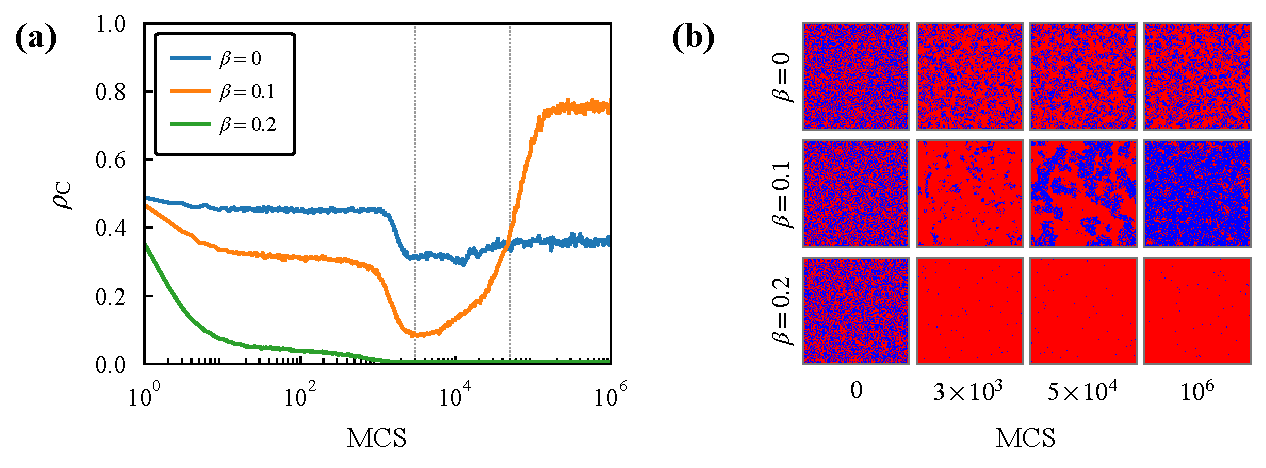
\includegraphics[width=\linewidth]{Fig_3.pdf}
\caption{
Temporal and spatial evolution of cooperation under different peer pressure intensities.
(a) Evolution of cooperation level $\rho_{\mathrm{C}}$ at $\beta=0$, $\beta=0.1$, and $\beta=0.2$.
(b) Corresponding spatial snapshots at $0$, $3000$, $50000$, and $1000000$ MCS, with rows representing $\beta=0$, $\beta=0.1$, and $\beta=0.2$, respectively.
Cooperators and defectors are represented by blue and red, respectively.
For each $\beta$, the trajectory and snapshots are obtained from the same simulation.
Vertical dotted lines in (a) mark the intermediate snapshot times.
The synergy factor and environmental threshold are fixed as $r=3.5$ and $T=3$, respectively, while other parameters are set to their default values.
}
\label{fig:Fig3}
\end{figure*}


\subsection{Peer pressure shapes the evolutionary dynamics and spatial organization of cooperation}

Figure~\ref{fig:Fig3} presents the temporal evolution of cooperation and the corresponding spatial patterns at $r=3.5$ and $T=3$, comparing the cases without pressure, with moderate pressure, and with strong pressure.

As shown in Fig.~\ref{fig:Fig3}(a), cooperation initially decreases in all three cases, with stronger pressure producing a faster decline. Without pressure, cooperation shows only a limited recovery. At $\beta=0.1$, cooperation reaches a lower minimum than without pressure but subsequently recovers to a higher level. At $\beta=0.2$, cooperation rapidly approaches zero. Moderate peer pressure therefore promotes cooperation recovery, whereas excessive pressure accelerates its loss and drives the population toward near-complete defection.

Figure~\ref{fig:Fig3}(b) shows the spatial changes accompanying these trajectories. At $\beta=0.1$, small cooperative clusters survive at $3000$ MCS and expand by $50000$ MCS, eventually occupying most of the lattice at $1000000$ MCS. At $50000$ MCS, cooperation levels at $\beta=0$ and $\beta=0.1$ are comparable. However, cooperators and defectors remain finely intermixed without pressure, whereas individuals adopting the same behavior aggregate into larger clusters at $\beta=0.1$. Under strong pressure, the lattice is already dominated by defection at $3000$ MCS, with only sparse cooperators remaining later. Moderate peer pressure thus favors the persistence and expansion of cooperative clusters, providing a spatial basis for cooperation recovery, whereas excessive pressure prevents the formation of extensive cooperative clusters.


\begin{figure*}[htbp]
\centering
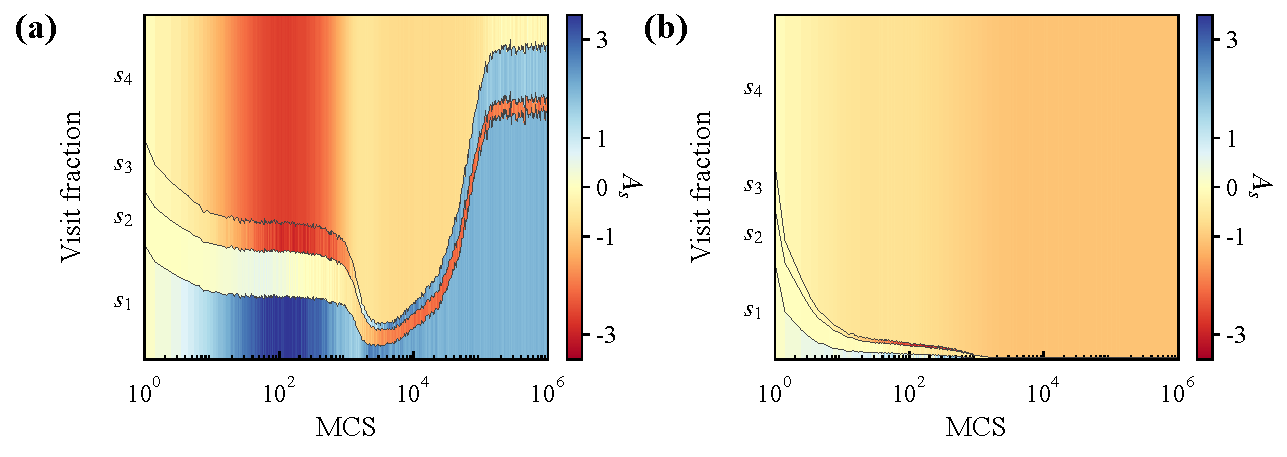
\includegraphics[width=\linewidth]{Fig_4.pdf}
\caption{
State visitation and learning dynamics under different peer pressure intensities. Band widths indicate state visit fractions, and colors represent the mean state-action advantage $A_s$ over actual visits. 
Panels (a) and (b) correspond to $\beta=0.1$ and $\beta=0.2$, respectively. 
All results are obtained with $r=3.5$ and $T=3$, while other parameters are set to their default values.
}
\label{fig:Fig4}
\end{figure*}


\subsection{Peer pressure shapes state-dependent learning}

To further understand why strong peer pressure suppresses cooperation, Fig.~\ref{fig:Fig4} examines state visitation and learning dynamics at $r=3.5$ and $T=3$. Band widths indicate state visit fractions, and colors represent the state-action advantage
\begin{equation}
A_s(t)=\left\langle Q_i(s,\mathrm{C})-Q_i(s,\mathrm{D})\right\rangle_{s,t},
\end{equation}
where $\langle\cdot\rangle_{s,t}$ denotes the average over actual visits to state $s$ during MCS $t$. Q-values are evaluated before the corresponding updates, and repeated visits by the same individual are counted separately. Positive and negative values of $A_s$ indicate an average preference for cooperation and defection, respectively.

Under moderate pressure, Fig.~\ref{fig:Fig4}(a) shows that $A_{s_1}$ increases rapidly during the early stage, while $A_{s_3}$ subsequently becomes positive. Cooperation thus becomes favored, on average, in both states associated with cooperative environments. Although the overall cooperation level initially declines, $s_1$ and $s_3$ continue to be visited. The surviving cooperative clusters shown in Fig.~\ref{fig:Fig3} provide local conditions for continued interactions in cooperative environments. When a group remains in a cooperative environment after action implementation, defectors receive pressure while cooperators are exempt. These interactions allow individuals to gradually develop cooperative preferences, including in $s_3$, where their current behavior is defection. The persistence of cooperative environments therefore retains learning opportunities that support subsequent cooperation recovery.

Under strong pressure, Fig.~\ref{fig:Fig4}(b) shows a rapid concentration of visits in $s_4$, which combines defection with a defective environment. With Q-values initially set to zero, the earliest updates are driven primarily by immediate rewards. Stronger pressure on cooperators in defective environments favors the early development of defection preferences, contributing to the faster decline of cooperation. Visits to $s_1$ and $s_3$ consequently become rare, leaving almost no opportunities for continued learning in cooperative environments. Meanwhile, $A_{s_4}$ remains negative, indicating a persistent preference for defection. Strong pressure thus accelerates the loss of cooperative environments, limiting the development of cooperative preferences and preventing subsequent cooperation recovery.


\begin{figure*}[htbp]
\centering
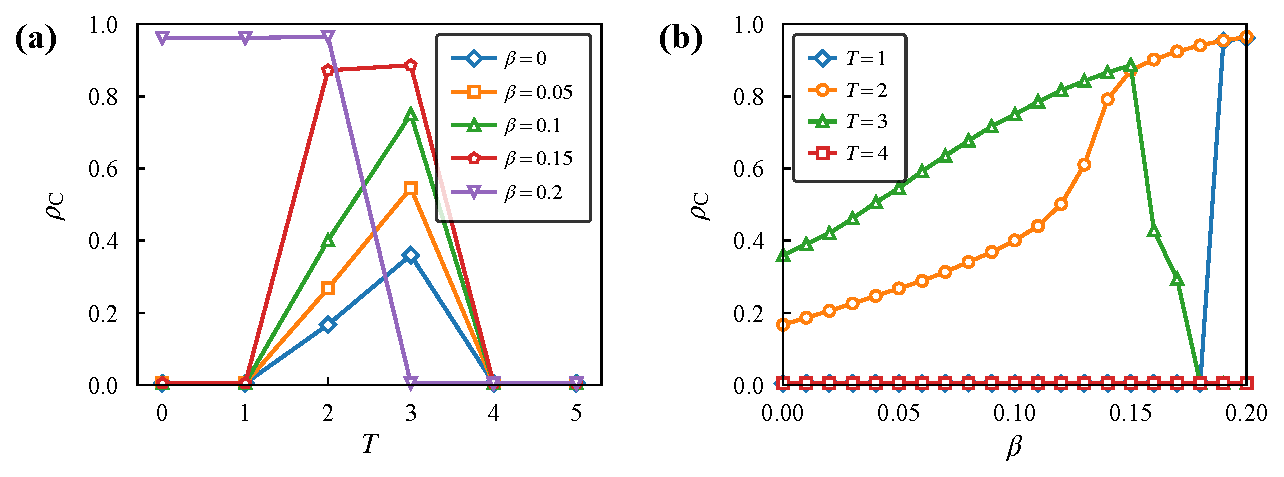
\includegraphics[width=\linewidth]{Fig_5.pdf}
\caption{
Effect of environmental threshold on cooperation. 
(a) Cooperation level $\rho_{\mathrm{C}}$ under different environmental thresholds $T$ and peer pressure intensities $\beta$. 
(b) Dependence of cooperation level $\rho_{\mathrm{C}}$ on $\beta$ at $T=1$, $2$, $3$, and $4$. 
All results are obtained with $r=3.5$, while other parameters are set to their default values.
}
\label{fig:Fig5}
\end{figure*}


\begin{figure*}[!t]
\centering
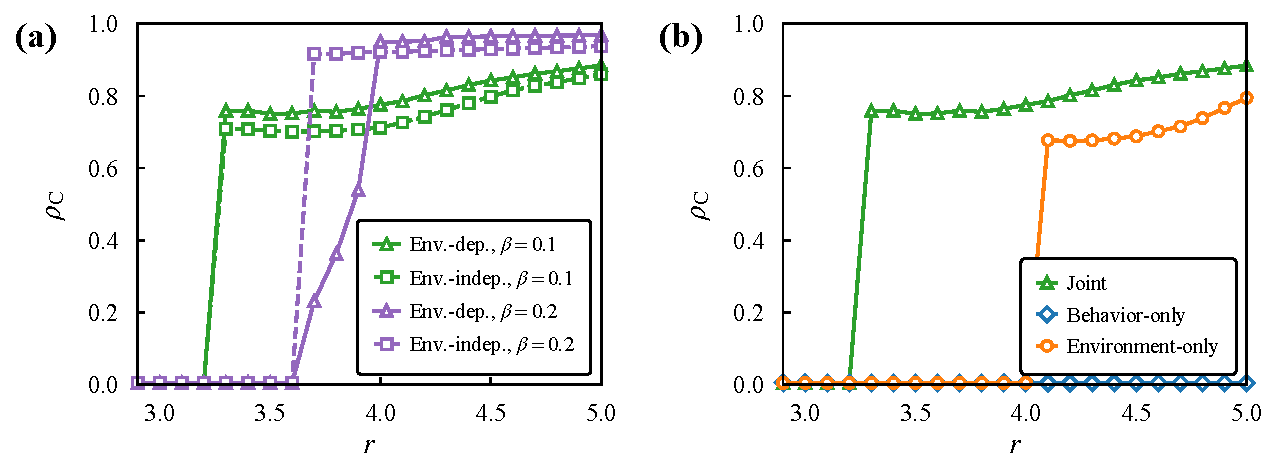
\includegraphics[width=\linewidth]{Fig_6.pdf}
\caption{
Effects of peer pressure rules and Q-table state representations on cooperation.
(a) Cooperation level $\rho_{\mathrm{C}}$ under environment-dependent pressure (solid lines) and environment-independent pressure (dashed lines), using the joint state representation at $\beta=0.1$ and $\beta=0.2$. Under environment-independent pressure, individuals receive pressure from all group members adopting the opposite action regardless of the group environment, while the learning states remain unchanged.
(b) Cooperation level $\rho_{\mathrm{C}}$ obtained using joint, behavior-only, and environment-only state representations under environment-dependent pressure at $\beta=0.1$.
The joint representation includes both individual behavioral and group environmental states.
All results are obtained with $T=3$, while other parameters are set to their default values.
}
\label{fig:Fig6}
\end{figure*}


\subsection{Environmental threshold shapes the response of cooperation to peer pressure}

We next examine how the environmental threshold $T$ affects cooperation at $r=3.5$. Figure~\ref{fig:Fig5}(a) shows that cooperation is highest at $T=3$, followed by $T=2$, under weak and moderate pressure. At $\beta=0.2$, high cooperation occurs at $T=0$, $T=1$, and $T=2$, whereas cooperation at $T=3$ is close to zero. At $T=4$ and $T=5$, cooperation remains close to zero for all pressure intensities shown. Threshold effects are also present at $\beta=0$, since environmental classification remains part of the learning state even without pressure. Thus, intermediate thresholds favor cooperation under weak and moderate pressure, whereas lower thresholds are more favorable under strong pressure.

Figure~\ref{fig:Fig5}(b) shows how cooperation responds to pressure at each threshold. At $T=1$, cooperation remains close to zero over most of the range but rises abruptly between $\beta=0.18$ and $\beta=0.19$. Cooperators are always exempt from pressure at this threshold, but defectors face only weak pressure when cooperators are scarce. Sufficiently strong pressure constrains defection and enables cooperation to emerge. At $T=2$, cooperation increases steadily with $\beta$. Only two cooperators are needed to form a cooperative environment, making this condition relatively easy to satisfy. Stronger pressure increases the cost of defection in these environments and favors cooperation. At $T=3$, cooperation peaks at $\beta=0.15$ and then falls close to zero at $\beta=0.18$. The spatial and learning dynamics underlying this response have been analyzed in Figs.~\ref{fig:Fig3} and~\ref{fig:Fig4}. At $T=4$, cooperation remains close to zero. Cooperative environments require at least four cooperators, exposing cooperators to pressure in a wider range of mixed groups and making cooperation difficult to sustain. These contrasting responses show that the threshold changes both the pressure needed to promote cooperation and the extent to which cooperation can withstand stronger pressure.


\subsection{Peer pressure rules and state representations affect cooperation evolution}

To examine the roles of the pressure rule and the information available for learning, we compare two pressure rules using the joint state representation and three state representations under environment-dependent pressure. The action space and learning parameters remain unchanged in these comparisons.

Figure~\ref{fig:Fig6}(a) compares environment-dependent pressure with environment-independent pressure, under which individuals receive pressure from all group members adopting the opposite action regardless of the group environment. Both rules retain the joint behavioral and environmental state representation. At $\beta=0.1$, environment-dependent pressure yields higher cooperation levels at $r$ values that support cooperation. At $\beta=0.2$, environment-independent pressure produces higher cooperation levels at $r=3.7$--$3.9$, whereas environment-dependent pressure yields slightly higher cooperation levels at larger $r$. The relative effects of the two rules therefore depend on both pressure intensity and the synergy factor.

The two rules differ in their allocation of pressure. Environment-dependent pressure exempts cooperators from pressure in cooperative environments, avoiding an additional payoff loss for cooperation. However, it also exempts defectors from pressure in defective environments, reducing the direct constraint on defection when cooperation is scarce. Environment-independent pressure removes both exemptions. These two effects help explain why environment-dependent pressure does not consistently yield higher cooperation than environment-independent pressure.

Figure~\ref{fig:Fig6}(b) compares the three state representations at $\beta=0.1$. With behavior-only states, cooperation remains close to zero throughout the examined range of $r$. With environment-only states, substantial cooperation appears only at $r=4.1$ and above. The joint representation supports high cooperation at lower $r$ and yields higher cooperation levels. The behavior-only representation retains the two states $\mathrm{C}$ and $\mathrm{D}$ but omits group environmental information, whereas the environment-only representation retains $\mathrm{G}$ and $\mathrm{B}$ but omits individual behavioral information. Retaining both types of information allows individuals to learn action values separately for different combinations of behavior and environment. These results show that distinguishing both individual behavior and group environment during learning helps sustain cooperation over a broader range of cooperation incentives.


\section{Conclusion}\label{sec4}

In this work, we have developed an environment-dependent peer pressure mechanism combined with a reinforcement learning framework in a spatial public goods game to investigate how environment-dependent social feedback influences the evolution of cooperation. 
The proposed framework allows peer pressure to exert different effects according to local environmental states, enabling individuals to adjust their behaviors under changing social conditions. 
By integrating environmental perception into reinforcement learning, our model provides a framework for understanding how local social information influences individual decisions and the evolution of cooperation.

Our results reveal several findings. 
First, the effect of peer pressure depends on its intensity, the synergy factor, and the environmental threshold. 
Under representative conditions, moderate pressure promotes cooperation, whereas excessive pressure accelerates the loss of cooperative environments and restricts opportunities for learning cooperative preferences, driving cooperation close to zero. 
This indicates that peer pressure intensity influences the evolution of cooperation by shaping learning feedback and subsequent strategy updates. 
Second, we find that higher synergy factors increase the tolerance of cooperative populations to stronger peer pressure, indicating that enhanced cooperative benefits help maintain cooperation under stronger social pressure. 
Third, the joint behavioral and environmental state representation supports higher cooperation than either simplified representation under the examined pressure condition. 
Retaining both types of information allows individuals to learn action values separately for different behavioral and environmental conditions and supports cooperation over a wider range of synergy factors.

These findings extend previous studies on social influence and cooperation evolution by showing that peer pressure does not have a universally positive or negative effect on cooperation evolution; instead, its evolutionary consequences depend on the interaction between pressure mechanisms, environmental conditions, and individual learning processes. 
The proposed framework highlights the importance of environment-dependent social feedback in sustaining cooperation and provides insights into how individuals adjust their decisions under different social conditions in real-world cooperative systems. 
Future studies could further incorporate more complex network structures~\cite{shi2024model}, heterogeneous learning abilities~\cite{lee2025granular}, and alternative state-transition rules~\cite{guo2022effect} to explore cooperation evolution under more realistic conditions.



\section*{Conflict of Interest}
The authors declare no commercial or financial relationships that could be construed as a potential conflict of interest.

\section*{Author Contributions}
\textbf{[To be completed after the author list is finalized.]}

\section*{Funding}
\textbf{[Funding information to be confirmed.]}

\section*{Acknowledgments}
The authors used OpenAI Codex (GPT-6.1 Sol; \url{https://openai.com/}) to assist with manuscript preparation and the development of simulation and plotting code. The authors reviewed and revised the outputs and take full responsibility for the content of this article.

\section*{Data Availability Statement}
The data that support the findings of this study are available from the corresponding author upon reasonable request.


% REVTeX's AIP substyle suppresses the bibliography heading by default.
\renewcommand{\bibsection}{\section*{References}}
\bibliographystyle{Frontiers-Vancouver}
\bibliography{ref}

\end{document}
%
% ****** End of file aipsamp.tex ******